\section{RC-Glied}

\subsection{Arbeitsgrundlagen}

Gem\"ass Theorie berechnet sich die Ausgangsspannung $U_A$ mit
\begin{equation}
    U_A = U_E \cdot \frac{X_C}{\sqrt{X_C^2+R^2}} = \frac{U_E}{\omega C \sqrt{\frac{1}{(\omega C)^2} + R^2}} = \frac{U_E}{\sqrt{1 + (\omega C R)^2}}
    \label{eq:ua}
\end{equation}

und die Phase $\varphi$ mit
\begin{equation}
    \varphi = \arctan(-\omega R C)
    \label{eq:phase}
\end{equation}


\subsection{Durchf\"{u}hrung}

\subsubsection*{Versuchsanordnung}

Am Eingang eines RC-Tiefpassfilters wurde eine sinusf\"ormige Wechselspannung mit Amplitude
$U_E = 4 V_{pp}$ und variabler Frequenz angelegt. Gemessen wurde die Ausgangsspannung $U_A$
sowie die Phasenverschiebung $\varphi$ in Funktion der Frequenz $f$ mit Hilfe eines
Kathodenstrahloszilloskopes (KO). Der Widerstand $R$ wurde zu $R=500\Omega$ bestimmt.
Die Messwerte wurden in der Tabelle \ref{tab:rc} aufgezeichnet.

\begin{figure}[H]
    \center
    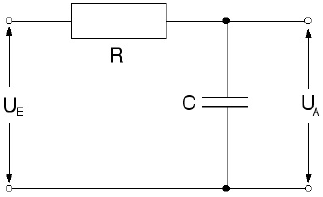
\includegraphics[width=.5\textwidth]{images/rc-lowpass}
    \caption{RC-Tiefpassfilter}
    \label{fig:rc}
\end{figure}


\subsubsection*{Messergebnisse}

\bgroup
    \setlength\tabcolsep{8mm}
    \begin{center}
        \begin{threeparttable}
            \caption{Gemessene Gr\"ossen}
            \begin{tabular}{ccc}
                \toprule
                $f(Hz)$  &  $U_a(V)$    &  $\phi$ \\
                \midrule
                100      & 4.000        & -3.24   \\
                500      & 3.800        & -16.9   \\
                1000     & 3.300        & -31.3   \\
                1500     & 2.800        & -43.6   \\
                5000     & 1.140        & -72.4   \\
                10000    & 0.580        & -82.5   \\
                100000   & 0.075        & -90.0   \\
                1592     & 2.700        & -44.0   \\
                \bottomrule
            \end{tabular}
            \begin{tablenotes}
                \small
                \item Messprotokoll ``Tiefpass''
                \item Datum: 1. Okt. 1999
                \item Versuchsleiterin: Ruth Metzler
                \item \textbf{Hinweis:} Daten wurden vom Auftragsdokument kopiert.
            \end{tablenotes}
            \label{tab:rc}
        \end{threeparttable}
    \end{center}
\egroup

Gesucht ist die Kapazit\"at $C$.


\subsubsection*{QtiPlot}

\begin{figure}[H]
    \center
    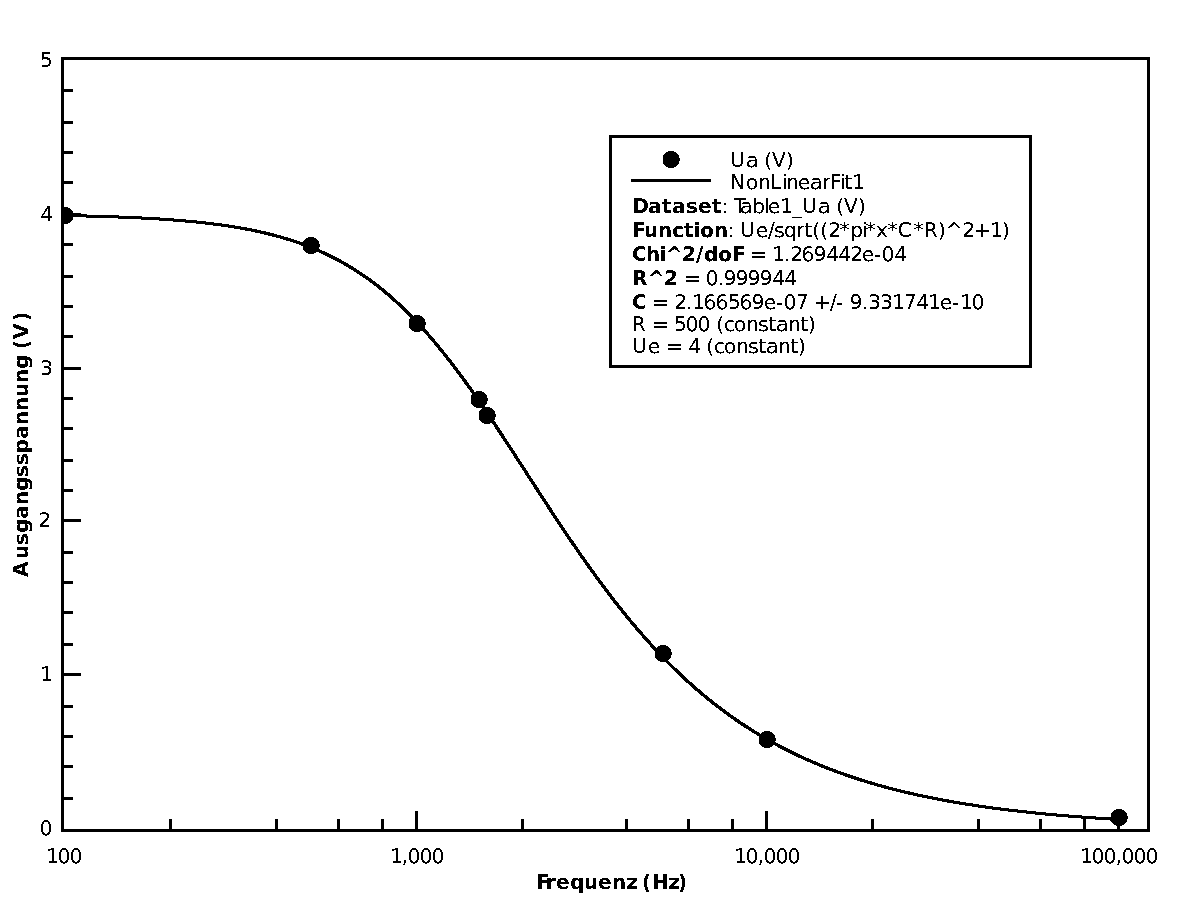
\includegraphics[width=.8\textwidth]{qtiplot/rc-ua}
    \caption{Nicht-lineare Regression zur Bestimmung von $C$ anhand der Ausgangsspannung}
    \label{fig:rc-ua}
\end{figure}

\begin{figure}[H]
    \center
    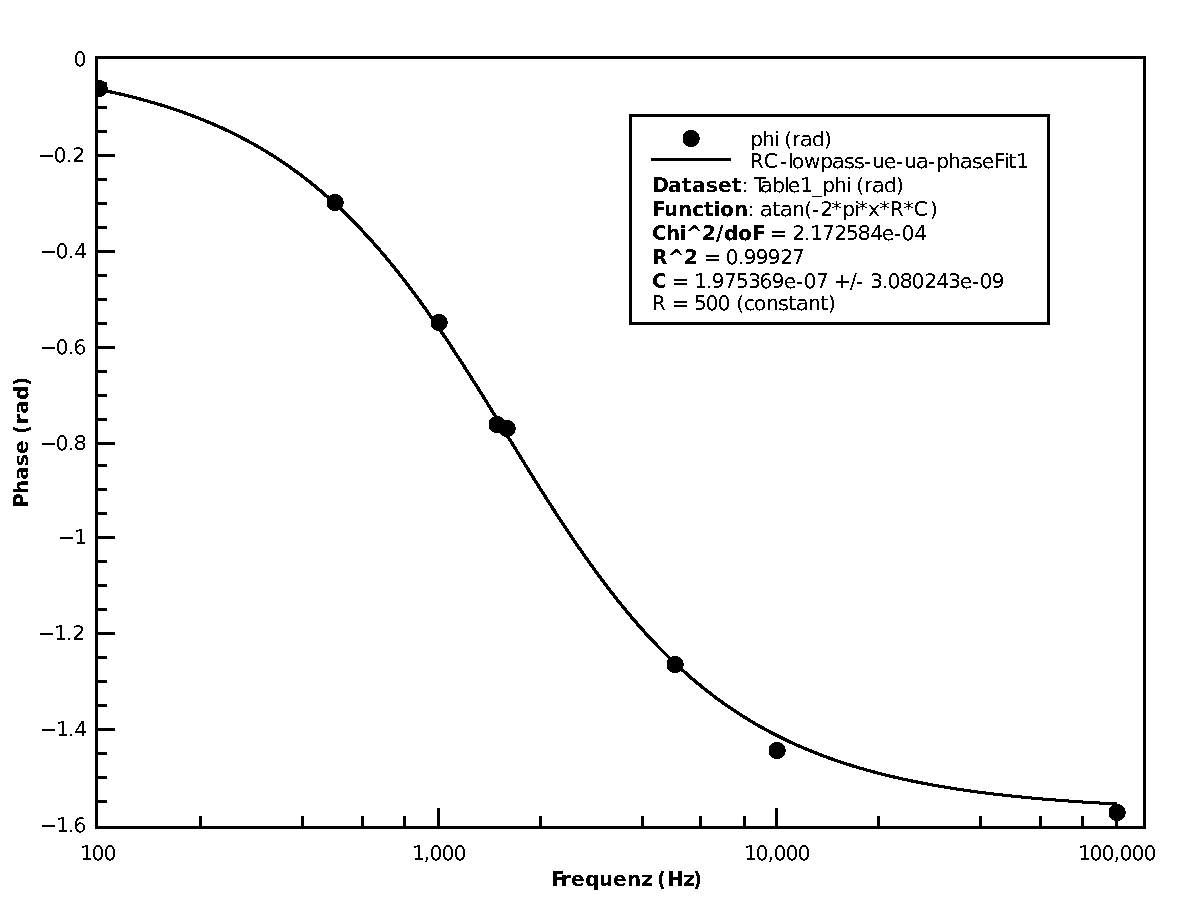
\includegraphics[width=.8\textwidth]{qtiplot/rc-phase}
    \caption{Nicht-lineare Regression zur Bestimmung von $C$ anhand der Phase}
    \label{fig:rc-phase}
\end{figure}


Die Kapazit\"at $C$ kann auf zwei Arten ermittelt werden.

\begin{itemize}
    \item In der Figur \ref{fig:rc-ua} wird die Ausgangsspannung $U_A$ in Funktion der Frequenz dargestellt.
    Durch Regression mit der Formel \ref{eq:ua} kann $C$ bestimmt werden. Der Wert betr\"agt somit
    $C_1 = (216.7 \pm 0.9)\SI{}{\nano\farad}$ (aus dem Plot von QtiPlot
    abgelesen).

    \item In der Figur \ref{fig:rc-phase} wird der Phasenwinkel $\varphi$ in Funktion der Frequenz dargestellt.
    Durch Regression mit der Formel \ref{eq:phase} kann $C$ auch bestimmt werden. Der Wert betr\"agt
    somit $C_2 = (197.5 \pm 3.1)\SI{}{\nano\farad}$ (aus dem Plot von
    QtiPlot abgelesen).
\end{itemize}


\subsection{Resultate und Diskussion}

Der Wert von $C_1$ weicht recht stark vom Wert $C_2$ ab. Es liegen sicher Messungenauigkeiten
zugrunde. Die Methode mit der Phase ist sicher ungenauer als die Methode mit der Ausgangsspannung,
weil die Phase $\varphi$ viel grober gemessen wurde. Dies reflektiert sich auch wenn man den Fehler
anschaut.

Um an einen genaueren Wert von $C$ zu gelangen k\"onnte man jetzt $C_1$ und $C_2$ gewichtet
mitteln mit
\begin{equation}
    \bar{C} = \frac{ \sum_{i=1}^{N} g_{\bar{C}_i} \cdot C_i }{ \sum_{í=1}^{N} g_{\bar{C}_i} }
            = \frac{ \frac{1}{0.9^2} \cdot 216.7 + \frac{1}{3.1^2} \cdot 197.5}{ \frac{1}{0.9^2} + \frac{1}{3.1^2} } = \SI{215.2}{\nano\farad}
\end{equation}
und den Fehler des gewogenen Mittels berechnen mit
\begin{equation}
    s_{\bar{C}} = \frac{1}{\sqrt{\sum_{i=1}^{N} g_{\bar{C}_i}}} = \frac{1}{\sqrt{\frac{1}{0.9^2} + \frac{1}{3.1^2}}} = \SI{0.9}{\nano\farad}
\end{equation}
Somit ergibt sich der genauere Wert $C = (215.2 \pm 0.9) \SI{}{\nano\farad}$

Es ist zu beachten, dass der berechnete Fehler der Kapazit\"at nur den statistischen Fehler
darstellt. Als systematischer Fehler m\"usste noch die Unsicherheit des Widerstandwertes
mitber\"ucksichtigt werden.

